\documentclass{article}

\usepackage{fancyhdr}
\usepackage{extramarks}
\usepackage{amsmath}
\usepackage{amsthm}
\usepackage{amsfonts}
\usepackage{tikz}
\usepackage[plain]{algorithm}
\usepackage{algpseudocode}
\usepackage{enumerate}
\usepackage{amssymb}

\usetikzlibrary{automata,positioning}

%
% Basic Document Settings
%

\topmargin=-0.45in
\evensidemargin=0in
\oddsidemargin=0in
\textwidth=6.5in
\textheight=9.0in
\headsep=0.25in

\linespread{1.1}

\pagestyle{fancy}
\lhead{\hmwkAuthorName}
\chead{\hmwkClass\ (\hmwkClassInstructor\ \hmwkClassTime): \hmwkTitle}
\rhead{\firstxmark}
\lfoot{\lastxmark}
\cfoot{\thepage}

\renewcommand\headrulewidth{0.4pt}
\renewcommand\footrulewidth{0.4pt}

\setlength\parindent{0pt}

%
% Create Problem Sections
%

\newcommand{\enterProblemHeader}[1]{
    \nobreak\extramarks{}{Problem \arabic{#1} continued on next page\ldots}\nobreak{}
    \nobreak\extramarks{Problem \arabic{#1} (continued)}{Problem \arabic{#1} continued on next page\ldots}\nobreak{}
}

\newcommand{\exitProblemHeader}[1]{
    \nobreak\extramarks{Problem \arabic{#1} (continued)}{Problem \arabic{#1} continued on next page\ldots}\nobreak{}
    \stepcounter{#1}
    \nobreak\extramarks{Problem \arabic{#1}}{}\nobreak{}
}

\setcounter{secnumdepth}{0}
\newcounter{partCounter}
\newcounter{homeworkProblemCounter}
\setcounter{homeworkProblemCounter}{1}
\nobreak\extramarks{Problem \arabic{homeworkProblemCounter}}{}\nobreak{}

%
% Homework Problem Environment
%
% This environment takes an optional argument. When given, it will adjust the
% problem counter. This is useful for when the problems given for your
% assignment aren't sequential. See the last 3 problems of this template for an
% example.
%
\newenvironment{homeworkProblem}[1][-1]{
    \ifnum#1>0
        \setcounter{homeworkProblemCounter}{#1}
    \fi
    \section{Problem \arabic{homeworkProblemCounter}}
    \setcounter{partCounter}{1}
    \enterProblemHeader{homeworkProblemCounter}
}{
    \exitProblemHeader{homeworkProblemCounter}
}

%
% Homework Details
%   - Title
%   - Due date
%   - Class
%   - Section/Time
%   - Instructor
%   - Author
%

\newcommand{\hmwkTitle}{Tutorial 4}
\newcommand{\hmwkDueDate}{February 9, 2021}
\newcommand{\hmwkClass}{CZ2003}
\newcommand{\hmwkClassTime}{SS3}
\newcommand{\hmwkClassInstructor}{Assoc Prof Alexei Sourin}
\newcommand{\hmwkAuthorName}{\textbf{Pang Yu Shao}}
\newcommand{\hmwkAuthorID}{\textbf{U1721680D}}

%
% Title Page
%

\title{
    \vspace{2in}
    \textmd{\textbf{\hmwkClass:\ \hmwkTitle}}\\
    \normalsize\vspace{0.1in}\small{Due\ on\ \hmwkDueDate\ at 10:30am}\\
    \vspace{0.1in}\large{\textit{\hmwkClassInstructor\ - \hmwkClassTime}}
    \vspace{3in}\\
    \hmwkAuthorName\\
    \hmwkAuthorID
}

\date{09/02/2021}

\renewcommand{\part}[1]{\textbf{\large Part \Alph{partCounter}}\stepcounter{partCounter}\\}

%
% Various Helper Commands
%

% Useful for algorithms
\newcommand{\alg}[1]{\textsc{\bfseries \footnotesize #1}}

% For derivatives
\newcommand{\deriv}[1]{\frac{\mathrm{d}}{\mathrm{d}x} (#1)}

% For partial derivatives
\newcommand{\pderiv}[2]{\frac{\partial}{\partial #1} (#2)}

% Integral dx
\newcommand{\dx}{\mathrm{d}x}

% Alias for the Solution section header
\newcommand{\solution}{\textbf{\large Solution}}

% Probability commands: Expectation, Variance, Covariance, Bias
\newcommand{\E}{\mathrm{E}}
\newcommand{\Var}{\mathrm{Var}}
\newcommand{\Cov}{\mathrm{Cov}}
\newcommand{\Bias}{\mathrm{Bias}}

\begin{document}

\maketitle

\pagebreak

\begin{homeworkProblem}
    \textbf{Using an equation in intercepts}, write an implicit equation of the plane
    which intersects the Cartesian coordinate axes X, Y and Z at three points with coordinates
    \(P_1=(1,0,0)\), \(P_2=(0,3,0)\), \(P_3=(0,0,6)\), respectively.
    \\

    \textbf{Solution}\\
    Implicit equation in intercepts:\\
    \(\frac{x}{a} + \frac{y}{b} + \frac{z}{c} = 1\)\\
    a = 1, b = 3, c = 6\\\\
    \(\therefore  \mathbf{f(x,y,z) = \frac{x}{1} + \frac{y}{3} + \frac{z}{6} - 1 = 0}\)    
    % \begin{figure}[H]
    %     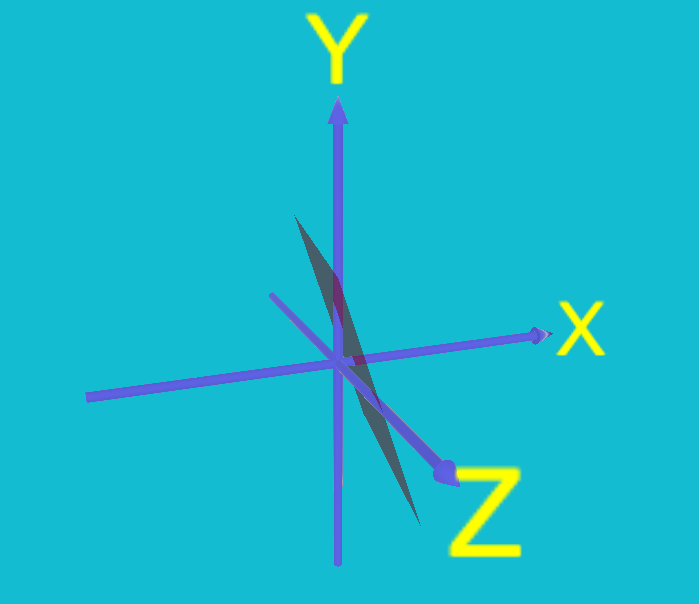
\includegraphics[width=8cm]{fig/q1.PNG}
    %     \centering
    % \end{figure}

\end{homeworkProblem}
\begin{homeworkProblem}
    Write an implicit equation of a plane which passes through the point with Cartesian coordinates 
    \((1,2,-3)\) while being orthogonal to the straight line defined by \(x=u+2\), \(y=u-1\), \(z=3u+1\),
    \(u \in (-\infty, \infty)\)\\

    \textbf{Solution}\\
    Normal vector to plane:\\
    \(\vec{N} = [A\ B\ C]\)\\
    \(\vec{N} = [1\ 1\ 3]\)\\\\
    Point on plane:\\
    \(r_o=(x_o, y_o, z_o)\)\\
    \(r_o=(1, 2, -3)\)\\\\
    Equation of a Plane (Point - Normal Form):\\
    \( A(x-x_0) + B(y - y_o) + C(z-z_0) = 0 \)\\\\
    \(\therefore \mathbf{f(x,y,z) =  (x-1) + (y - 2) + 3(z + 3) = 0} \)

    
\end{homeworkProblem}
\pagebreak
\begin{homeworkProblem}
    Propose how to define parametrically with functions \(x(u,v)\), \(y(u,v)\), \(z(u,v)\) a plane
    passing through points with coordinates \((-3,0,0)\), \((0,2,0)\), \((0,0,4)\).\\


    \textbf{Solution}\\
    To find a parametric equation of a plane with 3 points:\\
    \(P_1 + u(P_2 - P_1) + v(P_3 - P_1),\ \ u,v \in (-\infty, \infty) \)
    \\\\
    \(x(u,v) = x_1 + u(x_2 - x_1) + v(x_3 - x_1)\)\\
    \(y(u,v) = y_1 + u(y_2 - y_1) + v(y_3 - y_1)\)\\
    \(z(u,v) = z_1 + u(z_2 - z_1) + v(z_3 - z_1)\)\\
    \\\\
    \(x(u,v) = -3 + u(0 + 3) + v(0 + 3)\)\\
    \(y(u,v) = 0 + u(2 - 0) + v(0 - 0)\)\\
    \(z(u,v) = 0 + u(0 - 0) + v(4 - 0)\)\\
    \\\\
    \(\mathbf{x(u,v) = -3 + 3u + 3v}\)\\
    \(\mathbf{y(u,v) = 2u}\)\\
    \(\mathbf{z(u,v) = 4v}\)\\
    \(u,v \in (-\infty, \infty)\)


\end{homeworkProblem}
\pagebreak
\begin{homeworkProblem}
    A bilinear surface is defined by four points \(P1=(-1, 1, -1)\), \(P2=(1, 0, -1)\),
    \(P3=(-1, 0, 1)\) and \(P4=(1, 0.5, 1)\) and two parametric coordinates \(u \in [0,1]\)
    and \(v \in [0,1]\) , as illustrated in Figure Q3.
    \begin{figure}[H]
        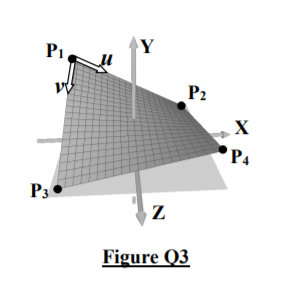
\includegraphics[width=6cm]{fig/q3.PNG}
        \centering
    \end{figure}
    \begin{enumerate}[(a)]
        \item Write parametric equations defining the bilinear surface.
        \item What are the coordinates of the point with the parametric coordinates 0.2, 0.4?
    \end{enumerate}

    \textbf{Solution}\\\\
    \textbf{a)}\\
    Bilinear Surface Parametric Representation:\\
    \( P = P1 + u(P2 - P1) + v(P3 - P1 + u(P4 - P3 – (P2 - P1) ) ),\ \ u,v \in [0,1] \)\\\\
    \( x(u,v) = x_1 + u(x_2 - x_1) + v(x_3 - x_1 + u(x_4 - x_3 – (x_2 - x_1) ) )\)\\
    \( y(u,v) = y_1 + u(y_2 - y_1) + v(y_3 - y_1 + u(y_4 - y_3 – (y_2 - y_1) ) )\)\\
    \( z(u,v) = z_1 + u(z_2 - z_1) + v(z_3 - z_1 + u(z_4 - z_3 – (z_2 - z_1) ) )\)\\\\
    \( x(u,v) = -1 + u(1 - (-1)) + v(-1 - (-1) + u(1 - (-1) – (1 - (-1)) ) )\)\\
    \( \mathbf{x(u,v) = 2u-1}\ \ u,v \in [0,1]\)\\\\

    \( y(u,v) = 1 + u(0 - 1) + v(0 - 1 + u(0.5 - 0 – (0 - 1) ) )\)\\
    \( \mathbf{y(u,v) = 1 -u -v + 1.5uv}\ \ u,v \in [0,1]\)\\\\

    \( z(u,v) = -1 + u(-1 - (-1)) + v(1 - (-1) + u(1 - 1 – (-1 - (-1)) ) )\)\\
    \( \mathbf{z(u,v) = 2v - 1}\ \ u,v \in [0,1]\)\\\\
    \pagebreak

    \textbf{b)}\\
    \(u = 0.2, v = 0.4\)


    \[
        \begin{split}
            x(0.2, 0.4)  &= 2(0.2) - 1
            \\
            &= - 0.6 
            \\
            y(0.2, 0.4)  &= 1 - 0.2 - 0.4 + 1.5*0.2*0.4
            \\
            &= 0.52
            \\
            z(0.2, 0.4)  &= 2(0.4) - 1
            \\
            &= - 0.2
            \\
            &
            \\
            \therefore P(0.2, 0.4) &= \mathbf{(-0.6, 0.52, -0.2)}
        \end{split}
    \]




\end{homeworkProblem}
\pagebreak
\begin{homeworkProblem}
    Write parametric equations \(x(u, v)\), \(y (u, v)\), \(z (u, v)\), \(u, v \in [0, 1]\) defining a
    triangular polygon which is bounded by the three segments defined by:\\\\

    \( x = 1 + 2 u \ \ \ \ \ \ y = 1 + u \ \ \ \ \ \ z = 1 - u \ \ \ \ \ \ u \in [0, 1] \)\\
    \( x = 3 - u \ \ \ \ \ \ \ y = 2 + u \ \ \ \ \ \ \ z = 4u \ \ \ \ \ \ \ \ \ u \in [0, 1] \)\\
    \( x = 2 - u \ \ \ \ \ \ \ y = 3 - 2u \ \ \ \ \ \ z = 4 - 3u \ \ \ \ u \in [0, 1] \)\\\\

    Finding vertices, let u = 0:\\
    \(P1 = (1, 1, 1)\)\\
    \(P2 = (3, 2, 0)\)\\
    \(P3 = (2, 3, 4)\)\\\\

    Bilinear Surface Parametric Representation:\\
    \( P = P1 + u(P2 - P1) + v(P3 - P1 + u(P4 - P3 - (P2 - P1) ) ),\ \ u,v \in [0,1] \)\\
    For triangle, let P3 = P4:\\
    \( P = P1 + u(P2 - P1) + v(P3 - P1 + u(P3 - P3 - (P2 - P1) ) ) \)\\
    \( P = P1 + u(P2 - P1) + v(P3 - P1 + u( P1 - P2 ) ) \)\\\\

    \( x(u,v) = 1 + u(3 - 1) + v(2 - 1 + u( 1 - 3 ) ) \)\\
    \( \mathbf{x(u,v) = 1 + 2u + v(1 - 2u)} \)\\\\

    \( y(u,v) = 1 + u(2 - 1) + v(3 - 1 + u( 1 - 2 ) ) \)\\
    \( \mathbf{y(u,v) = 1 + u + v(2 - u)} \)\\\\

    \( z(u,v) = 1 + u(0 - 1) + v(4 - 1 + u( 1 - 0 ) ) \)\\
    \( \mathbf{z(u,v) = 1 - u + v(3 + u)} \)\\\\
    \(\mathbf{u,v \in [0,1]}\)






\end{homeworkProblem}

    



\end{document}